\chapter{Evaluation}
\label{section:results}

In the following section we will compare the different algorithms in three different experiments.
Each experiment will be described, the results will be presented and interpreted.
First we will look at two fairly simple environments, one that acts in discrete space and one that acts in continuous space.
These environments are used to better understand the algorithms used in this thesis.
In the end we will look at the actual problem of this paper, the application of these algorithms on the snake-like environment.
Note that all graphs in this section are smoothed by a Savitzky-Golay-Filter for better display.

\section{CartPole-v0}

The first environment we chose was the \emph{CartPole-v0} environment.
Table \ref{tb:cartpole_specs} shows the specification of this environment.

\begin{table}[H]
  \centering
  \begin{tabular}{| c | c |}
      \hline
      Observation space & Continuous\\
      \hline
      Num Observations & $4$\\
      \hline
      Action Space & Discrete\\
      \hline
      Num Actions & $2$\\
      \hline
  \end{tabular}
\caption{Specification of the CartPole-v0 environment}
\label{tb:cartpole_specs}
\end{table}

\subsection{Goals}

The objective of the CartPole-v0 is to balance a pole on a cart that can move left or right.
This is a discrete problem because we can either push left with full force or right with full force.
In the beginning of each episode the cart is spawned in the center of the screen and the pole is initialized with a small random angle..
The agent receives $1$ reward for every time step it keeps the pole balanced.
An episode terminates if the pole falls too far to one side or the cart moves too far to one side.
It is solved when obtaining an average return of $195$ over $100$ consecutive episodes.
We chose this environment to start off with because it is a discrete environment with only two actions and only four observations.
It is considered a very easy to solve environment.
DQN is known to act better in discrete action spaces which makes this environment a perfect fit.
This was the first environment we trained our first algorithm on and was more of a testing stage for later problems to come.

\subsection{Realization}

We'll run our algorithms for 1000 episodes which corresponds to roughly 1 hour of training.
The data will be collected by simply cumulating all rewards we observed in one episode.
At first we will run the basic DQN and then add all extensions to it and run it again.
Table \ref{tb:dqn_params} shows the hyperparameters we'll use for the DQN with and without extensions.

\begin{table}[H]
  \centering
  \begin{tabular}{| c | c |}
      \hline
      Hyperparameter & Value\\ \hline
      Layer 1 size & $20$\\
      Layer 2 size & $20$\\
      Batch size & $20$\\
      Target Update Freq. & $50$\\
      $\alpha$ & $0.00025$\\
      $\gamma$ & $0.9$\\
      $\epsilon$ & $0.1$\\
      \hline
  \end{tabular}
\caption{Hyperparameter configuration for Dueling DQN with PER}
\label{tb:dqn_params}
\end{table}


\subsection{Results}

\begin{figure}[H]
\centerline{
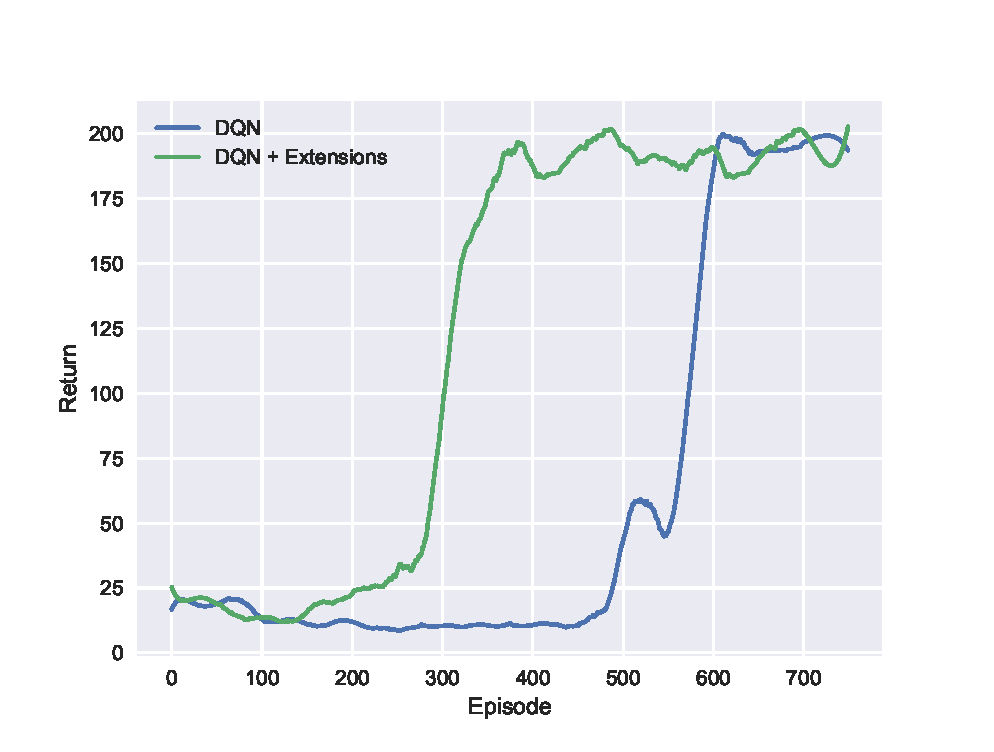
\includegraphics[width=0.7\textwidth]{images/dqn_compare_cartpole.eps}}
\caption{Comparison of the algorithms on the CartPole-v0 environment}
\label{fig:cartpole_compare}
\end{figure}

Figure \ref{fig:cartpole_compare} shows the results for this environment.
As one can see the steep learning curve appears around 200 episodes earlier when extensions are applied.
Because all hyperparameters were the same in both runs it is clear that the extensions actually have a positive impact on the learning curve.
In our experiment the DQN with extensions solved the environment after around 400 episodes while the basic DQN took around 700 episodes to solve it.
This means that the extensions required around 40\% less training data to solve the environment.


\section{Pendulum-v0}

Next we move from the discrete action-space of the CartPole-v0 environment to the continuous
action-space of the Pendulum-v0 environment.
Table \ref{tb:pendulum_specs} shows the specifications of this environment.

\begin{table}[H]
  \centering
  \begin{tabular}{| c | c |}
      \hline
      Observation space & Continuous\\
      \hline
      Num Observations & $3$\\
      \hline
      Action Space & Continuous\\
      \hline
      Action Dimensions & $1$\\
      \hline
  \end{tabular}
\caption{Specification of the Pendulum-v0 environment}
\label{tb:pendulum_specs}
\end{table}

\subsection{Goals}

The goal of this environment is to swing up a pendulum and then balance it.
The agent can achieve this by applying a force to the pendulum pushing it either to the left or to the right.
In the beginning of each episode the pendulum is initialized in a random position.
Each episode terminates exactly after $200$ timesteps.
The agent receives a small negative reward in each timestep corresponding to the degree it is off from balancing it straight up.
E.g. if it hangs loosely downwards it would be 180° off which is the worst possible position.
With this environment we want to make a smooth transition from the easy discrete environment of the CartPole-v0 to our continuous snake-like environment.
The Pendulum-v0 is still a considerably simple to solve environment but as already mentioned acts in a continuous space.
We want to see from this experiment which algorithms are worth trying on the snake-like environment.

\subsection{Realization}

In this experiment we will use the same hyperparameters for DQN as before.
We will only run the version with extensions applied.
Again the data will be collected by simply cumulating all rewards we observe in one episode.
All algorithms will run for just 200 episodes.
Table \ref{tb:ddpg_params} shows the hyperparameters we'll use for all our DDPG experiments.
We will look at how DQN performs on this task and then compare it to DDPG with and without parameter noise applied.

\begin{table}[H]
  \centering
  \begin{tabular}{| c | c |}
      \hline
      Hyperparameter & Value\\ \hline
      Layer 1 size & $200$\\
      Layer 2 size & $200$\\
      Batch size & $32$\\
      Learning Rate Actor & $0.0001$\\
      Learning Rate Critic & $0.001$\\
      Replay Memory Size & $1000000$\\
      $\tau$ & $0.001$\\
      \hline
  \end{tabular}
\caption{Hyperparameter configuration for DDPG}
\label{tb:ddpg_params}
\end{table}

\subsection{Results}

\begin{figure}[H]
\centerline{
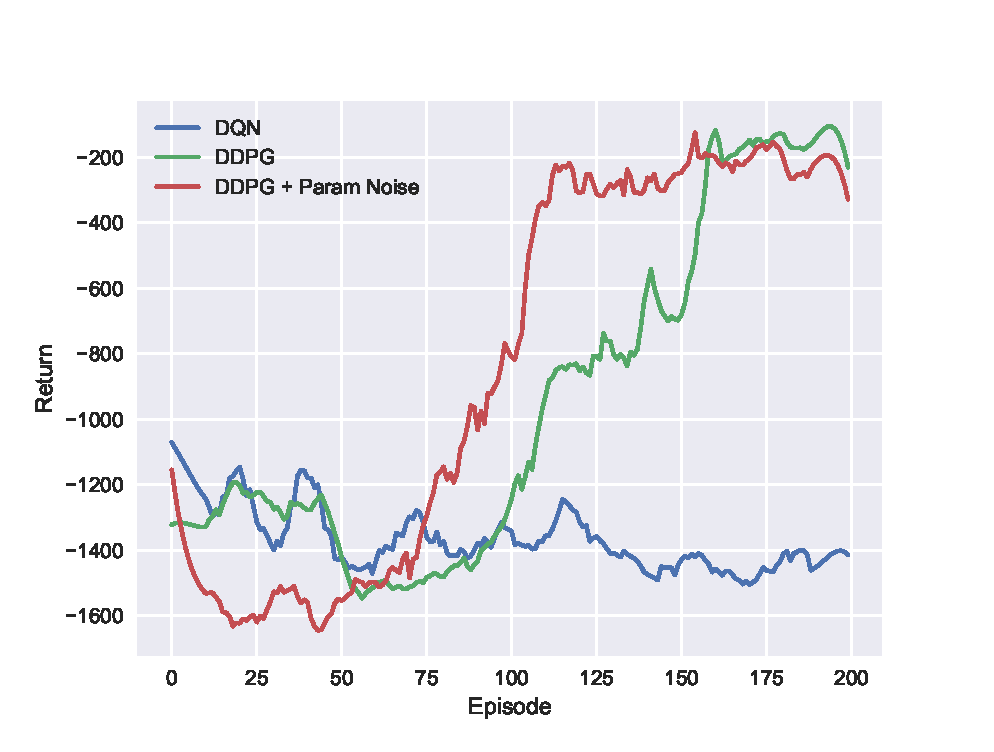
\includegraphics[width=0.7\textwidth]{images/pendulum_compare.eps}}
\caption{Comparison of the algorithms on the Pendulum-v0 environment}
\label{fig:pendulum_compare}
\end{figure}

Figure \ref{fig:pendulum_compare} shows the results for all three runs in this environment.
Unfortunately DQN failed to learn a useful policy on this task.
DDPG on the other hand learned a good policy after only 200 episodes of training and adding parameter
noise to it returned even better results. Because the DQN failed on this task
already we decided not to try it on the snake as the Curse of Dimensionality [1] makes it
an even harder problem for DQN.

\section{Swimmer-v1}

After successfully solving the Pendulum-v0 we now move on to the Swimmer-v1 environment.
This environment is the main environment of this thesis because it represents a snake-like robot very closely.
It has two joints that can be moved in any direction to produce movement. Table \ref{tb:swimmer_specs} shows the specifications for this environment.

\begin{table}[H]
  \centering
  \begin{tabular}{| c | c |}
      \hline
      Observation space & Continuous\\
      \hline
      Num Observations & $8$\\
      \hline
      Action Space & Continuous\\
      \hline
      Action Dimensions & $2$\\
      \hline
  \end{tabular}
\caption{Specification of the Swimmer-v1 environment}
\label{tb:swimmer_specs}
\end{table}


\subsection{Goals}

The goal is to move the robot as far to the right as possible. The agent receives a small positive or negative reward in each timestep according to a reward function that takes into account the position of the snake relative to the starting point and the smoothness of the movement.
With this experiment we want to see which algorithm produces the best results on a snake-like robot.
We also want to look at our new way of introducing noise to the PPO.

\subsection{Realization}

We'll again use the same hyperparameters for DDPG as before and again compare DDPG with and without action noise.
At first we will only look at PPO without additional noise factors and later compare those results separately.
We will run all our experiments on this environment for $1500$ episodes.
Note that it makes a significant difference in computational time whether to use DDPG or PPO.
While DDPG takes around 10 seconds per episode, PPO takes nearly no time for a single episode and only takes around a few seconds of training time after one trajectory.
Table \ref{tb:ppo_params} shows the hyperparameters used for all PPO experiments.
\begin{table}[H]
  \centering
  \begin{tabular}{| c | c |}
      \hline
      Hyperparameter & Value\\ \hline
      Layer 1 size & $100$\\
      Layer 2 size & $100$\\
      Trajectory size & $5$\\
      Learning Rate Actor & $0.00025$\\
      Learning Rate Critic & $0.0025$\\
      $\gamma$ & $1$\\
      $\lambda$ & $0.98$\\
      $\epsilon$ & $0.2$\\
      \hline
  \end{tabular}
\caption{Hyperparameter configuration for PPO}
\label{tb:ppo_params}
\end{table}

\newpage

\subsection{Results}

\begin{figure}[H]
\centerline{
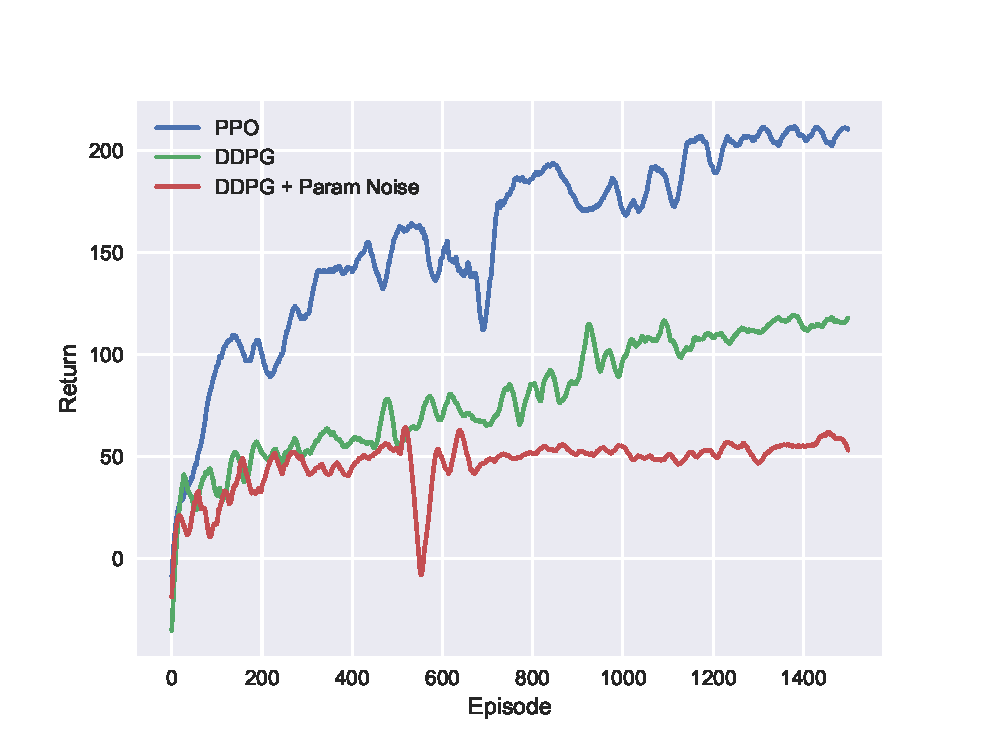
\includegraphics[width=0.7\textwidth]{images/snake_compare.eps}}
\caption{Comparison of the algorithms on the Swimmer-v1 environment}
\label{fig:snake_compare}
\end{figure}

Figure \ref{fig:snake_compare} shows all results of our different algorithms.
As one can see the DDPG gets stuck in a local maximum after some time at around 120. This is a known problem
for DDPG algorithms when dealing with more complex problems. Although the variance
of different runs is pretty small for the DDPG. This means that on every run it settles at a
score of around 120 after 1000 to 1500 episodes. For some reason adding parameter noise
to it now makes the performance way worse. We were not able to reproduce the desired
results of the original paper for this environment.


PPO is better and settles at a score of around 200 after 1500 episodes. The problem here
is that the variance for PPO is very high. In these graphs we only include the best runs of
all algorithms.

\newpage

\begin{figure}[H]
\centerline{
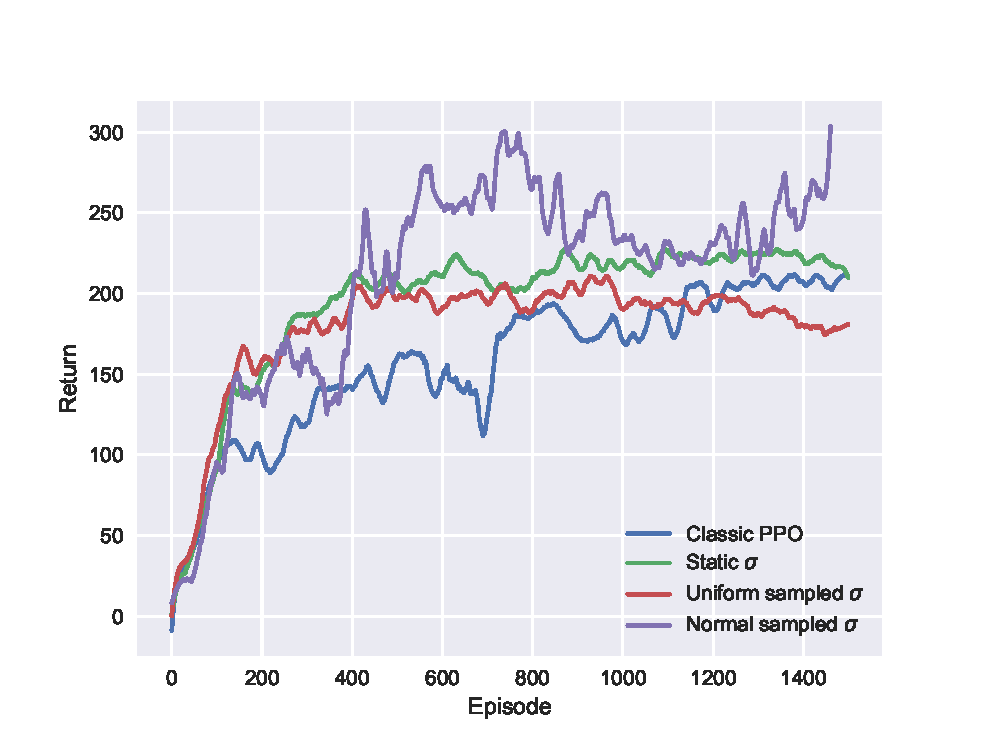
\includegraphics[width=0.7\textwidth]{images/ppo_compare_noise.eps}}
\caption{Comparison of different noise factors}
\label{fig:ppo_noise_compare}
\end{figure}

Lastly we compared our different approaches to add noise to the PPO.
Figure \ref{fig:ppo_noise_compare} shows the best runs for all algorithms.
The graph for classic PPO is the same as in Figure \ref{fig:snake_compare} and is only added to give a reference to the other graphs.
Keeping the standard deviation static seems to be a little more stable and settles after only 400 episodes at a score of 200.
Sampling from a uniform distribution before every trajectory makes no difference compared to the classic PPO.
By sampling the standard deviation from a normal distribution though we achieved a score of over 300 after 1500 episodes.
This is a significant improvement towards the classic PPO algorithm and all of our other approaches.
The high achievement in the beginning of the learning process can probably be linked to better exploration.


In this chapter we set up three different experiments for all the algorithms.
We started off by looking at fairly simple problems at first before moving on to the more complex problem of the snake-like robot.
In the end we also looked at our new way of introducing noise to PPO and compared different ways to do so.
In the next section we will conclude the findings of this thesis and present future work.
